\chapter{Experimental Setup and Evaluation}
\begin{comment}

    Experimental Setup and Evaluation

- Goal of Experiment
- Methods and actual tools used
- Experimental Setup in detail
- Experimental procedure
- Presentation of experimental results

update to overleaf since git is not working!

\end{comment}

This chapter will go over the experimental aspect of this work including the tools and equipment used to implement the algorithms. The setup of the experiments and the testing done on each algorithm and the process of developing these algorithms. The benchmarking results for the two discovery algorithms will be discussed.

We will also present the experimental results for the two algorithms as a proof of concept for the algorithms as presented in the previous chapter.



\section{Equipment and Modeling}
The FESTO water management system was designed for educational purposes in automation. For this work it was equipped with two sensors and three actuators. All of the capabilities of these sensors and actuators are exposed as web resources on three NodeMCU ESP8266 microcontrollers following the Web of Things architecture. Below is the mapping of the microcontrollers to their actuators. In addition to each of the capabilities of their mapped actuators each microcontroller exposes the resources \texttt{/urdfl} and \texttt{/urdfq}, allowing the device to load and query RDF data respectively. In this case the NodeMCU 3 has been mapped multiple devices.

\vspace{1cm}
\begin{figure}[ht]
\centering
\begin{tabular}{l | l}
  water level sensor (LUT400) & NodeMCU 1 \\
  flow sensor (Sitrans F M Mag 6000) & NodeMCU 2 \\
  on/off valve & NodeMCU 3 \\
  pump on/off switch & NodeMCU 3 \\
  water heater on/off switch & NodeMCU 3 \\
\end{tabular}
  \caption{Mappings of Servients to Sensors \& Actuators}
  \label{table:mappings}
\end{figure}

The FESTO unit was originally built as a pedagogical tool to help engineers learn about automation. Here it serves as a minimal viable model of a water reclamation facility. Because the benchmarks only required the semantic data, it was unnecessary to use the FESTO unit while conducting the tests. Instead each experiment was conducted on a with the three NodeMCUs connected to a PC.

\begin{figure}[th]
\centering
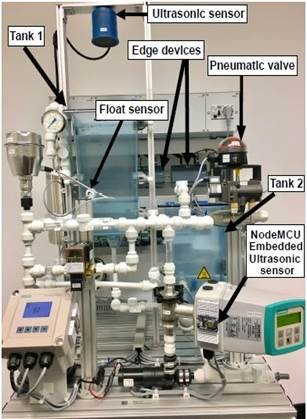
\includegraphics[width=.7\textwidth]{Figures/festoDemonstrator.jpg}
\caption{The FESTO Demonstrator}
\label{fig:festoDem}
\end{figure}



\section{Tools Used}



\subsection{Apache Jena}

Apache Jena is a Java framework used to build Semantic Web applications. It entails various APIs, which work together to process RDF, OWL, and SPARQL. The centralized discovery algorithm required Apache Jena in order to manipulate blank nodes.

There are several modules within Apache Jena, in this paper the most  used was the Core RDF API. In the Core RDF API RDF Graphs can be represented by the data structure \texttt{Model}, which is composed of \texttt{Statements} or may be implemented in the simpler and more limited Java API \texttt{Graph}. \texttt{Statements} entailing one subject, predicate, and object represent a \textit{triple} and are immutable in Jena. This means triple had to be altered when piecing together connected graphs, such as in the \textt{GraphLean} algorithm, the new \textt{Statement}s had to be created with the updated information and the old Statement could then be removed from the \textt{Model} and the new one appended. This process was not included in the benchmarking times, since took place on a PC and the primary interest was the amount of time message passing required. \cite{Jena.24.10.2017}

\subsection{ESP8266}

The ESP8266 is an inexpensive Wi-Fi capable system on a chip (SoC) manufactured by the Chinese company Espressif. It fully supports the TCP/IP stack and 802.11 b/g/n/d/e/i/k/r. The ESP8266 has a small amount of flash memory available--only about 512 kB, though this can be upgraded to 4 MB. The algorithms created in this work were tested using the NodeMCU version of this chip, which includes a special firmware for IoT development. \cite{Zeroday.2017}


This microcontroller is unquestionably rugged: it has an operating temperature range spanning from -40\textdegree{}C to 125\textdegree{}C and is therefore suitable for a wide spectrum of applications. It can be used for home applications, including home automation: monitoring home appliances, monitoring the energy output of photovoltaic cells, managing lights and outlets, baby monitors, etc. It's wide operating temperature range also makes it an appropriate choice in industrial wireless control networks and sensor networks. \cite{espDatasheet} Additionally the ESP8266 has a modest price and is available starting at 5 EUR if purchased individually, with bulk pricing hovering at around 1 EUR per unit. \change{citation needed?}

There are several versions of firmware publicly available for the ESP8266, Siemens created its own version based off of the NodeMCU firmware. A key feature of the NodeMCU firmware is the integration of embedded Lua (eLua) \cite{Zeroday.2017}, which entails the same features as the desktop version plus additional features useful for embedded developers. Like Lua, eLua is able to run on nearly every platform, because it was implemented in ANSI C. \cite{Marinescu.}

Lua is an extensible language, meaning it can integrate functions, which cannot (or should not) be directly written in Lua. This works using the C API, which allows code written in C to interact with Lua. The C API is also available in eLua. The combination of the simplicity and high-level abstraction of a scripting language with the portability and light-weight implementation in C \cite{luaHandbook}, means eLua is powerful tool for embedded developers. This work used Lua in the distributed discovery algorithm.
% https://nodemcu.readthedocs.io/en/master/en/upload/ TODO: continue



\change{removed other picture of NodeMCU, add your own picture of ESP8266, others are copyrighted}

\subsection{ESPlorer}
ESPlorer is an IDE used by ESP8266 developers. It can run on Windows, Linux, MacOS, and Solaris and it provides tools for working in Lua for the NodeMCU and MicroPython. For benchmarking it was run in a virtual machine running Ubuntu 16.04.

\begin{figure}[h]
\centering
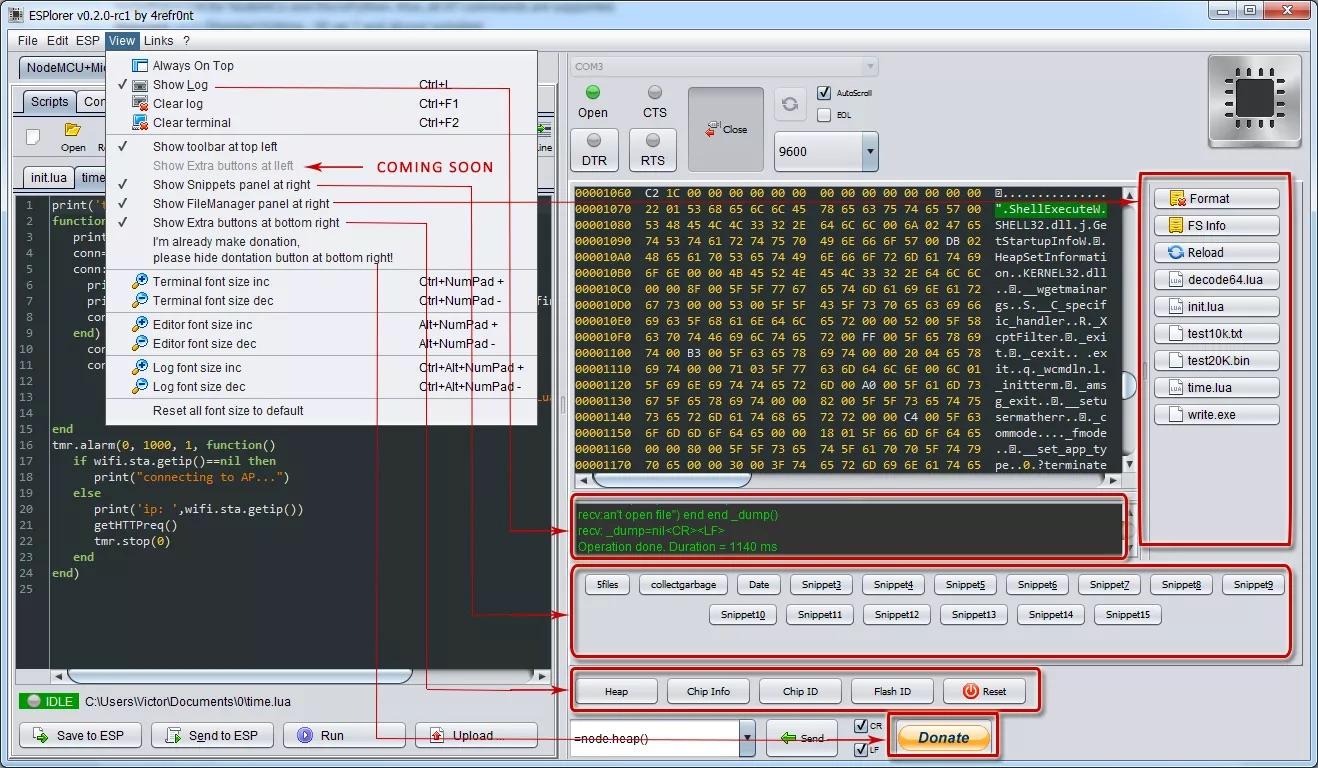
\includegraphics[width=\textwidth]{Figures/ESPlorer.jpg}
\caption{The ESPlorer interface. Image is from the NodeMCU documentation\cite{Zeroday.2017}}
\end{figure}

Code is written in the buffer on the left, while the right buffer shows the current status and connection to the NodeMCU. Connecting to the NodeMCU is simple: after plugging the NodeMCU in, users hit the refresh button in the upper-right corner, then select the COM port, and finally the baud rate.

After a connection to the NodeMCU has been established, code can be simply added and removed from the NodeMCU using buttons in the lower left side of the IDE.

\section{Experimental Procedure}

The modified REDD algorithm was implemented in Java using Apache Jena.

The centralized discovery algorithm also used Jena to compose and send SPARQL queries. \change{come back to this}

This section will outline the implementation details for the algorithm implementations from this work, specifically how they were implemented, how they were tested, and how they were benchmarked.

\subsection{The REDD Algorithm}


The REDD algorithm was vital to the centralized discovery. Since the REDD Algorithm as presented by Esposito et al. was incorrect, we wanted to ensure what we contributed delivered what was intended. Our version of the REDD algorithm was verified by unit testing with JUnit. This includes checking that the queries that were created were created from the models were converted correctly. This was especially important when forming queries containing blank nodes.


Other JUnit tests were created to test the correctness of the algorithms using trivial dummy RDF graphs. This ensured that the resultant blank RDF node pairs computed by the algorithm were in fact correct. Unit tests checked that the blank node connected graphs were created correctly and that the redundant blank node pairs were correct.

Since we had the pseudocode from Esposito (Figure \ref{fig:EspositoListing}), this was used as a framework for our implementation. First the simpler algorithms were implemented, like the \texttt{ExecuteQuery} and the \texttt{BuildConnGraphs} functions. This was estimated to take about two weeks--but ended up requiring more than three months, since the original paper did not contain adequate information to recreate the algorithm and contained definitions from the W3C recommendations used without any further explanation. Other than that the article was vague and even incorrect as submitted, according to one of the paper's co-authors.

Lastly a data type for the connected graphs (\texttt{ConnectedGraph}) was created, as well as a data type for the pairs of \texttt{RDFNode}s, called \texttt{RDFNodePair}.

\begin{figure}[h]
\centering
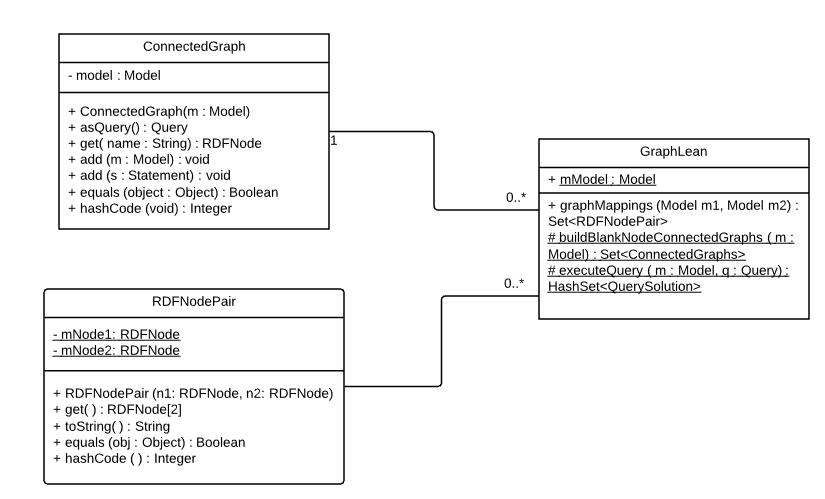
\includegraphics[width=\textwidth]{Figures/REDDuml.png}
\caption{The UML diagram of the implemented REDD Algorithm.}
\end{figure}

We started by implementing the the pseudocode as it was likely intended to be implemented: one graph was processed and searched for redundant subgraphs. As discrepancies came up in the implementation, we reached out to the author, but since the paper was so old (2005), the author no longer had any code and expressed that she neither had the "time, nor the interest" in discussing the algorithm further. So left to our own devices, we rebuilt the algorithm, as we thought was intended and verified using unit testing.

Once the REDD algorithm was implemented as it was in most likely intened in Espoisto's paper, we changed the graph mappings function, to run queries between to graphs, $G_1$ and $G_2$. Finally, this algorithm could be used to update graphs in the centralized discovery algorithm.


\subsection{The Centralized Discovery}

The set-up for the centralized discovery was quite simple: the three NodeMCUs are connected to a PC, which acts as the client.

Each iteration of the centralized discovery can be broken down into two steps: (1) the semantic graphs are combined (2) the resultant lean graphs are sent to the respective servient. Benchmarks measured the time it took for the graphs to be processed with the REDD algorithm and the amount of time it took for the graphs to be sent to the servients, the latter being especially relevant for this work. The former is largely dependent on hardware capability and is not particularly noteworthy.

\change{add activity diagram}

\change{too concise, add more detail}

Between each iteration the times were recorded in a table. \change{expand}


To asses whether the order of the NodeMCUs affected the total time for the discovery algorithm, the benchmark was run ten times with each permutation of the semantic data. Therefore the benchmark ran 60 times in total.



\subsubsection{Results}


\subsection{The Decentralized Discovery}
The decentralized discovery was very simple to implement, but did require the semantic data to be prepared for the algorithm.

The semantic data was converted from the RDF/XML serialization to the EXI format.\change{was also converted to thingy}




The decentralized discovery has a similar setup to the centralized benchmark. All three of the NodeMCUs were connected to a computer. The computer was running a Linux VM. In the VM there were three instances of ESPLorer \change{talk about ESPLorer}

Each NodeMCU was loaded with firmware, which contained a way to store and query RDF data. Each NodeMCU also was loaded with its semantic data in a binary format, Efficient XML, EXI, which was used because requires less broadband and can be processed faster. \cite{} \change{make citation of W3C rec for EXI} \change{EXI is not talked about before, consider discussing in foundations}

In this benchmark there were two quantities we were interested in: the time taken to complete each message pass and the payload size of each message.


\subsubsection{Results}
The original idea of the decentralized discovery was to multicast a query to all nodes. This idea proved to be improbable because of message collisions and timeouts, due to the exposed node problem. \change{flesh me out} Instead of using a multicast IP each NodeMCU had a neighborhood list of the IP addresses in the network and sent queries individual neighbors. In a later implementation, staggering the multicast times on each NodeMCU using a random timer also worked, but rather unreliably. \change{word for one-after-the-other?}


\section{Future Work}

Due to time and scope constraints there are several things that were not accomplished in this work. The REDD algorithm, as implemented here, has quite a few weaknesses regarding blank node management. When we followed up with Luigi Iannone, a co-author of the REDD paper \cite{Esposito.2005}, he recommended another approach using A-Box logic to cull blank nodes. He claimed, that the time savings were not as expected and more importantly that it broke semantic data, when used in datasets with multiple ontologies. This means that the proposed algorithms in this work are not robust.

Regarding the discovery algorithms, the decentralized discovery would be vastly improved if the exposed node problem could be worked around, so that the multicast address could be used in lieu of querying all the neighbors in the neighborhood list. Of course this problem is not just limited to our application, but is a broader problem in wireless sensor networks and ad-hoc systems. By integrating solutions from these frameworks, the decentralized discovery's reliability may be improved. \change{be sure to go into more detail, don't be afraid to write your thoughts on this, pick 1/2 papers and go for it}

The experiment discussed in this paper only examined three microcontrollers, yet scalability is a key challenge to the successful industrial application of these algorithms. Running experiments in scalability will be necessary to have a solid proof of concept. Ideally networks should be tested with 100s or 1000s of nodes. Without suitable hardware simulators, benchmarking this is quite difficult.

In an industrial setting the performance of discovery algorithms applied to mobile devices is especially interesting. For example tracking mobile robots, such as restocking robots, or wearables on employees track of the position of workers on the factory floor, could help to avoid dangerous accidents with heavy machinery. This requires flexible, autonomous reconfiguration of the network. Adding the new device is easier than removing the devices semantic data from the network, so each time the network should remove a device, the web of semantic data would have to be rebuilt from the ground-up. One solution could be taken from relational databases: semantic data that should be deleted could be flagged as inactive, like when an employee leaves after his shift, and then upon arrival in the area his semantic data could be unflagged.
